
\documentclass[twocolumn, twoside,a4paper,10pt]{article}
\pagestyle{plain}
\addtolength{\textheight}{2cm}
\includeonly{expmeth}

\usepackage{amsmath, amsthm, amsfonts}
\usepackage{graphicx}
\usepackage[show]{ed}

%---------------------------------------------------------------------
\title{\textbf{Superconductivity and Electron Tunneling}}
\author{Thomas McColgan and Miguel Garc\'ia Echevarr\'ia\\
	\small{\textit{Laboratorio de Bajas Temperaturas, Dpto. de F�sica de la Materia Condensada}} \\
	\small{\textit{Facultad de Ciencias, UAM}}
	}
\date{Madrid, \today}
%---------------------------------------------------------------------
\begin{document}
%-----------------------------------------------------------------
%-----------------------------------------------------------------
%ABSTRACT
\twocolumn[ 
\begin{@twocolumnfalse} 
\maketitle % need full-width title 
\begin{abstract} 
\small{We repeat the 1960 experiment by Giaver, in which the tunneling current from a superconductor through an insulating film is measured to obtain the width of its gap. Our results and the discrepancies to the BCS Theory are discussed. We measure the lead energy gap to be $(1.4 \pm 0.1)$ meV for $T<4.2\ K$}.
\vspace{1cm}
\end{abstract}
\end{@twocolumnfalse}
]

%-----------------------------------------------------------------
%-----------------------------------------------------------------
\section{Introduction}

% === Introduction ===

This is the introduction! Yes!

%Motivation(BCS predicts Gap)
The theory of superconductivity presented by Bardeen, Cooper and Schrieffer in 1957 predicts a gap in the allowed energies for electrons. Even though this gap had been measured indirectly by several methods, it had not been measured directly until Giaver conducted his electron tunneling experiment, which we have attempted to reproduce here.

%Historical Context(Giaver, Nobel)



%-----------------------------------------------------------------
%-----------------------------------------------------------------
\section{Theoretical Approach}
%---------------------------------------------------------------------------------------
\begin{frame}
\frametitle{Efecto t�nel cu�ntico}
Explicar simplemente el efecto t�nel cu�ntico... 

F�rmula, quiz� s�lo la dependencia de la anchura y del potencial...

\end{frame}
%---------------------------------------------------------------------------------------
%---------------------------------------------------------------------------------------
\begin{frame}
\frametitle{}

\end{frame}
%---------------------------------------------------------------------------------------
%---------------------------------------------------------------------------------------
\begin{frame}
\frametitle{}

\end{frame}
%---------------------------------------------------------------------------------------
%---------------------------------------------------------------------------------------
\begin{frame}
\frametitle{Densidad de estados para los 3 tipos de uniones}

\begin{figure}[h!]
\centering
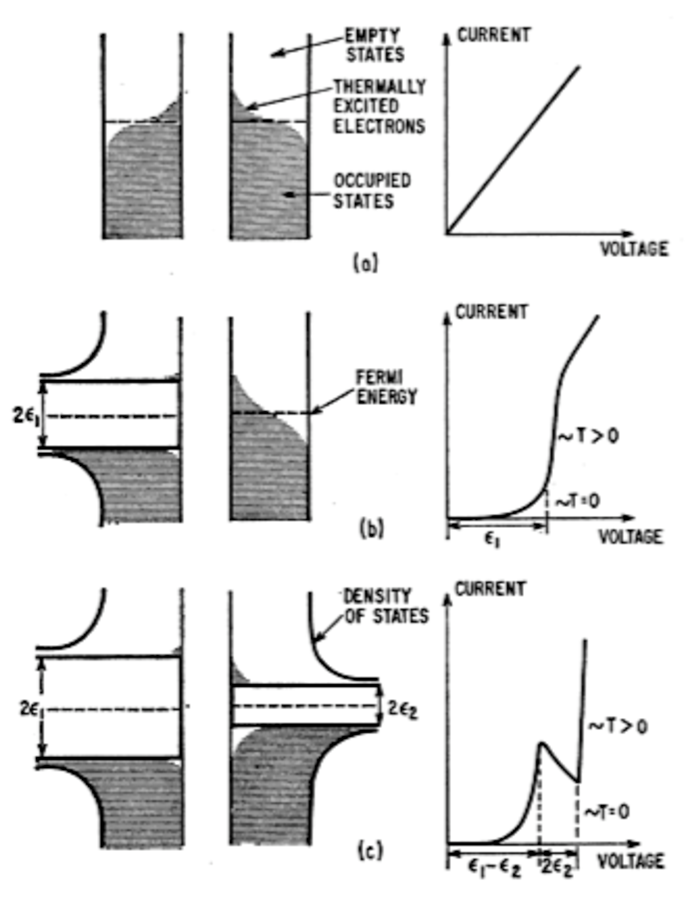
\includegraphics[width=0.6\textwidth]{fermi_levels}
%\caption{\small Densidad de estados para los 3 casos
%\label{fermi_levels}}
\end{figure}

\end{frame}
%---------------------------------------------------------------------------------------
%---------------------------------------------------------------------------------------
\begin{frame}
\frametitle{}

\end{frame}
%---------------------------------------------------------------------------------------
%---------------------------------------------------------------------------------------
\begin{frame}
\frametitle{}

\end{frame}
%---------------------------------------------------------------------------------------
%---------------------------------------------------------------------------------------
\begin{frame}
\frametitle{}

\end{frame}
%---------------------------------------------------------------------------------------
%---------------------------------------------------------------------------------------
\begin{frame}
\frametitle{}

\end{frame}
%---------------------------------------------------------------------------------------
%---------------------------------------------------------------------------------------
\begin{frame}
\frametitle{}

\end{frame}
%---------------------------------------------------------------------------------------

%-----------------------------------------------------------------
%-----------------------------------------------------------------
\section{Experimental Method}
%Experimental Methods

Our aim in this experiment was to measure superconductor to normal tunneling as described above. To achieve this we choose Aluminum as the superconductor and Lead as the normal conductor. This is convenient because $Al$ and $Pb$ have a transition temperature of $1.140 K$ and $7.193 K$ respectively. Therefore the range in between the two allows the observation of the desired effect. Another benefit is that Aluminum readily oxidizes to $Al_2O_3$ at room temperature, providing an insulating layer.\\

\subsection{Sample Preparation}
Sample preparation was done in a manner similar to the one described in \ref{giaever1}. First a thin layer of Aluminum was vapor-deposited by means of a heated spiral filament onto a microscope slide in a vacuum chamber. Air was then let into the chamber, allowing a thin insulating film of $Al_2O_3$ to form. Finally the chamber was evacuated again, and the last layer, consisting of $Pb$, was deposited.\\

%SLIDE LAYOUT GRAPHIC\\
\begin{figure}
\centering
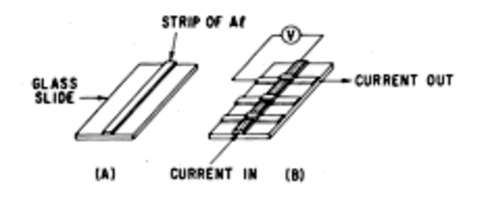
\includegraphics[scale=1]{sample.pdf}
\caption{Hola\label{sample}}
\end{figure}


The layers were deposited in the shape of strips, a long strip of $Al$ crossed by 5 shorter strips of $Pb$, providing up to 5 tunnel junctions per slide. The shapes of the layers were determined by placing a mask between the heated filament and the slide.\\

\todo{Say something about the layer thickness, ways of estimating it.} \\

There are 2 main reasons for preparing the samples in a vacuum. Firstly it is necessary to keep the layers as free from contamination as possible, because due to their thinness even small amounts of foreign substances might cause a change in behavior. Secondly the vacuum significantly reduces scattering effects, making the thickness of the deposited layers as homogenous as possible. This is necessary so that the current is distributed evenly across the junction.\\

We used an oil diffusion pump to attain a high vacuum of about\ednote{get value from cuaderno} bar.\\

\subsection{Measurement}
The sample was immersed in a cryostat containing liquid $He$ surrounded by a layer of liquid $N$. A rotary pump was connected to the cryostat to reduce pressure inside. Since the vapor pressure is linked to the temperature of the Helium this allowed us to perform measurements at several temperatures. A mechanical manometer was also connected to the chamber.\\

\begin{figure}
\centering
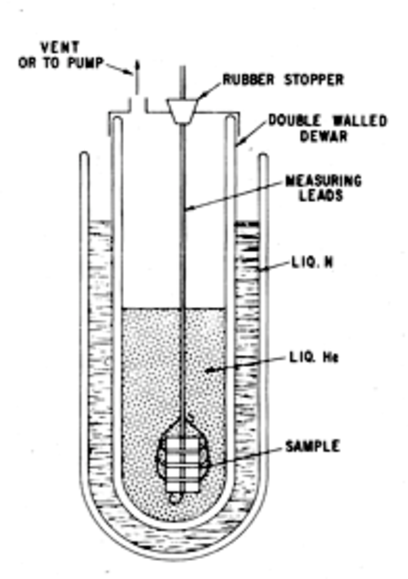
\includegraphics[scale=0.6]{cryostat.pdf}
\caption{Hola\label{cryostat}}
\end{figure}

%MYSTERY: $p_{bottom} = p_{top}$?\\

The tunnel junction was connected in a 4 terminal configuration, i.e. the voltage and current were measured in two separate circuits, which only joined at the tunneling junction. This setup has the advantage that only the potential difference at the junction itself is measured, and factors such as the resistivity of cables leading up to the sample, and the change with temperature thereof, do not have to be taken into account. \\

In our setup the Ampere-meter also functioned as a current source. Both units were connected to a computer via an IEEE interface, which was used to set the current and record the readings. In each measurement run the voltage across the junction was measured for a range of equally spaced current intensities, as produced by said current source.  We measured ranges from\ednote{get values from cuaderno} to using divisions between 100 and 2000 steps. A time of $1s$ was left between measurements to allow for the readings to stabilize.

The resolution of voltage measurements depended greatly on the range in which the measurement was taken. The Volt-meter automatically changes the resolution, therefor we tried to avoid such changes of resolution by setting corresponding limits on the current. When the data contained a change of scale we omitted the data points beyond the change. The effects of this change of resolution are most severe in the numerical derivation, since this is done by dividing the differences.

%In order to measure the effect described above in the case of normal-superconductor tunneling, we prepare samples of two metals with different transition temperatures separated by an insulator. We vapor-deposited thin layers of aluminum and lead on a microscope glass slide,  leaving the Aluminum layer at the open air for a short period to let some insulating $AlO_2$ oxide form.

%IT HAS TO BE CLEAR THAT WE HAVE A SANDWICH!!!!!!!

%1) sample preparation: vacuum chamber (torr?? why?? mean free path), filament, layer thickness (method for calculating it: isotropy or resistance? Justify that the second one gives smaller thickness with Poisson distribution, because we have rare events), ... HOW MUCH/MANY?????!!!!!!!!!!!!!!

%2) Cryostat, nitrogen, helium, vacuum pump, manometer, T-P of vapor-pressure He, why don't we have different P's up and down in the cryostat? The T is different... And... HOW MUCH???

%3) Measurement: 4 terminals (why? HOW MUCH?), constant steps sized intensity, 


%-----------------------------------------------------------------
%-----------------------------------------------------------------
\section{Results and Analysis}

\subsection{Data Analysis}

\begin{figure}[b!]
\centering
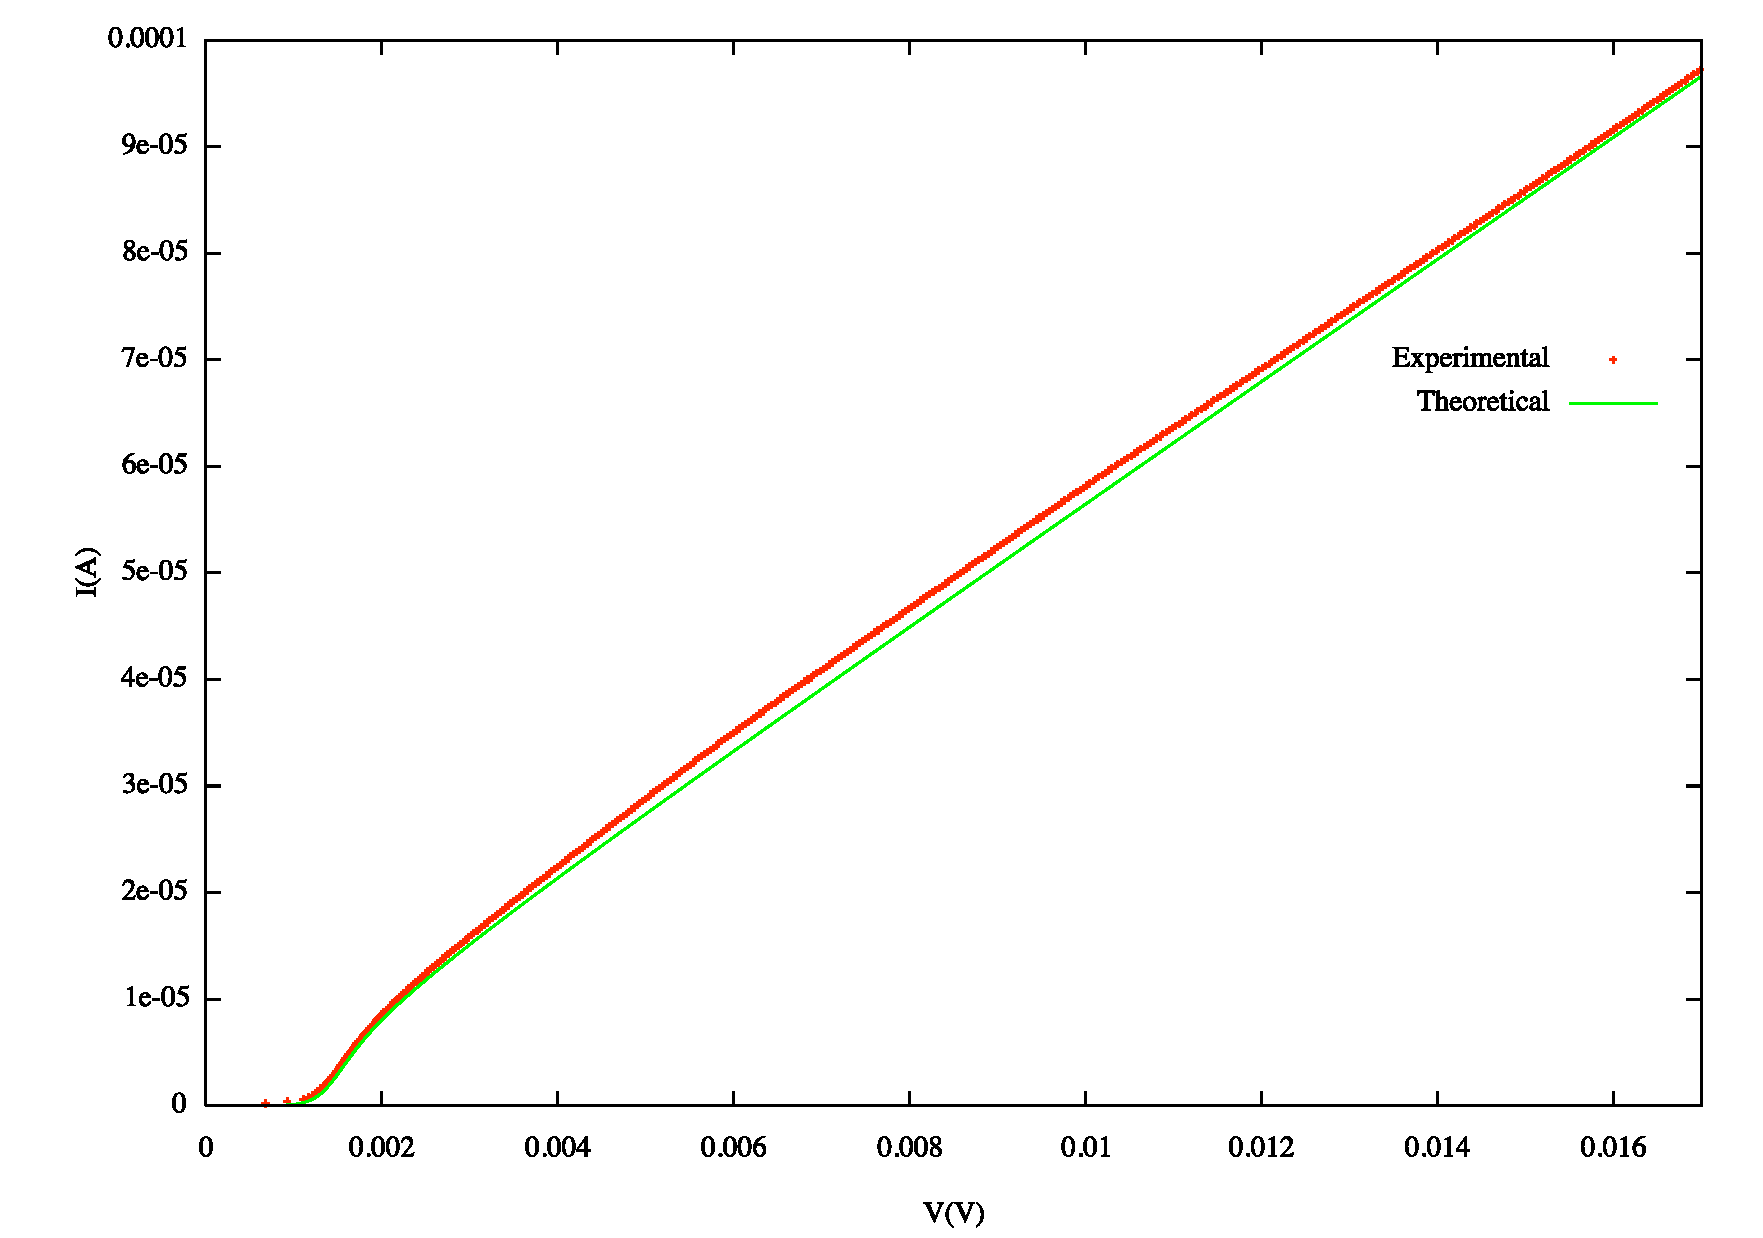
\includegraphics[width=0.45\textwidth]{iv-7-exp_theo}
\caption{\small Experimental data and BCS theoretical prediction for $1.45 K$. The different density of states of Pb with respect to BCS causes the discrepancy. 
\label{iv-7-exp_theo}}
\end{figure}

Our first step in analyzing the collected data was to plot it. Since the shape of the energy spectrum is given by the derivative of the I-V curve, it was necessary to numerically calculate the derivative. The method we chose to do this was to fit a linear function to $n$ neighboring data points using a straightforward least squares approach. The slope of the fitted function was taken as the derivative.This had the additional benefit of performing some smoothing. Of course there is some information lost in the process, but this was not deemed critical as the number of points collected was generally much larger than $n$.

In order to estimate the energy gap of our Pb sample it was necessary to evaluate the integral in \ref{ins_numerical}, 
\begin{eqnarray*}\label{ins_numerical2}
I^{NS} &=& \frac{C^{NN}}{e} \int_{0}^{\infty} dx\ \frac{x+\Delta}{\sqrt{x(x+2 \Delta)}} \times
		\nonumber \\
		&\times& [f(x+ \Delta-eV)-f(x+ \Delta +eV)],
		\nonumber \\
\end{eqnarray*}
and compare the results to the experimental data. To do so we split the integral in 2 parts. The high energies were evaluated numerically using a Romberg-Method algorithm \cite{recipes}, while the lower energies were estimated analytically. It was assumed that $ [f(x+ \Delta-eV)-f(x+ \Delta +eV)] \approx \text{const.}$ for small $x$, as it is finite and nonzero for $x=0$, while the other part, $\frac{x+\Delta}{\sqrt{x(x+2 \Delta)}}$, diverges for $x\to0$. It can, however, be integrated analytically up to $0$, thus enabling us to efficiently integrate for all $x$. 
\begin{equation*}\label{num}
 \int_{0}^{a} dx\ \frac{x+\Delta}{\sqrt{x(x+2 \Delta)}} = \sqrt{a(2\Delta+a)}
\end{equation*}

To get the conductance curve, the resulting theoretical I-V curve was derivated in the same manner as the experimental data, i.e. with the same degree of smoothing, to ensure their comparability.

\begin{figure}[h!]
\centering
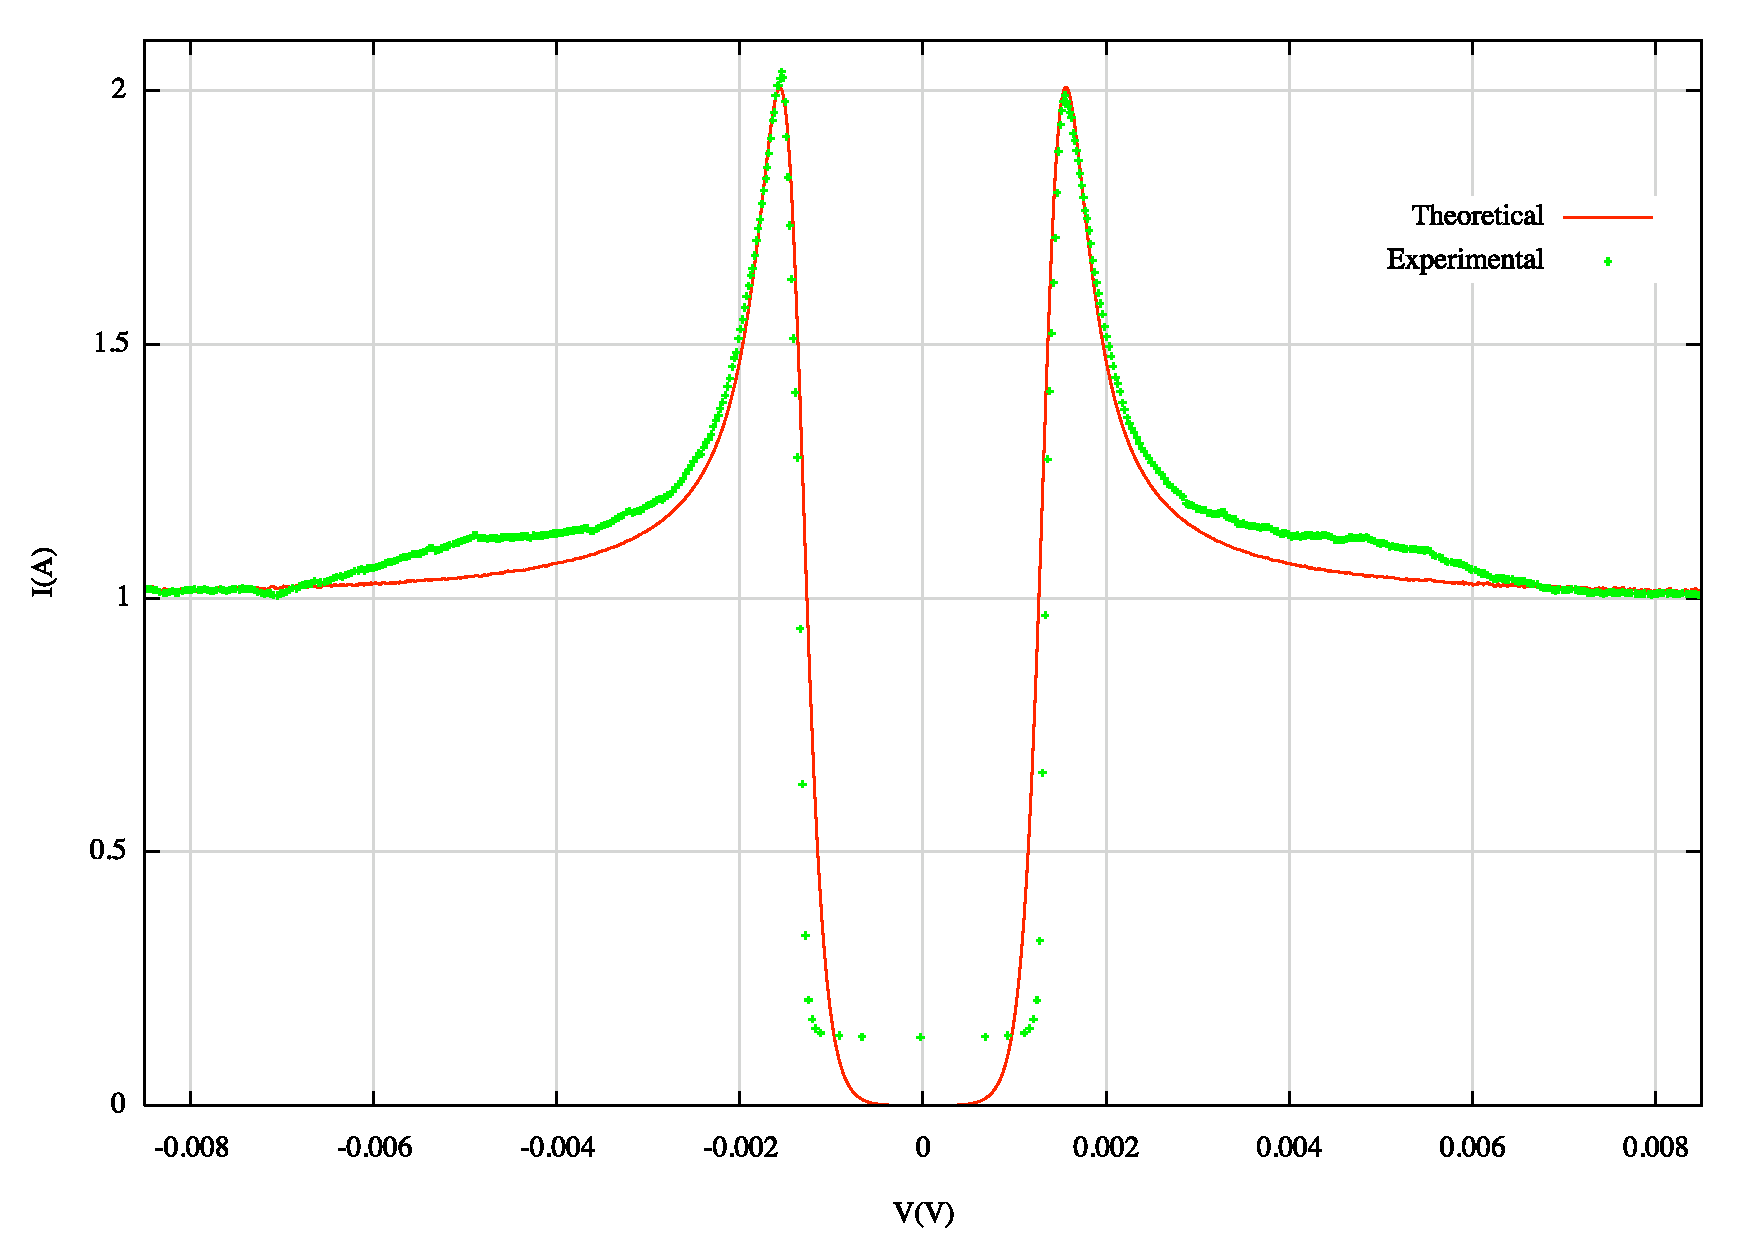
\includegraphics[width=0.45\textwidth]{gv_theo_exp_7}
\caption{\small Experimental data and BCS theoretical prediction for Conductance at $1.45 K$. The discrepancy in I-V curve in fig. \ref{iv-7-exp_theo} has its corresponding here. The numerical derivation smoothes more significantly experimental data than theoretical ones near $0V$ due to points density. The peaks are smoothed more equally.  
\label{gv_theo_exp_7}}
\end{figure}

%1.- BCS does not fully describe the measured data. The density of states is different... --> Residual
When plotting the derivatives in this way and comparing them qualitatively to each other for some arbitrary but reasonable values of $T$,$\Delta$ and $C_{NN}$ it quickly becomes apparent that there are certain qualitative differences between the experimental results and the results predicted by the BCS theory. Specifically, there are some bulges in the conductance curves outside the gap in the experimental data which are not present in the theory (see fig. \ref{gv_theo_exp_7}).

\begin{figure}[h!]
\centering
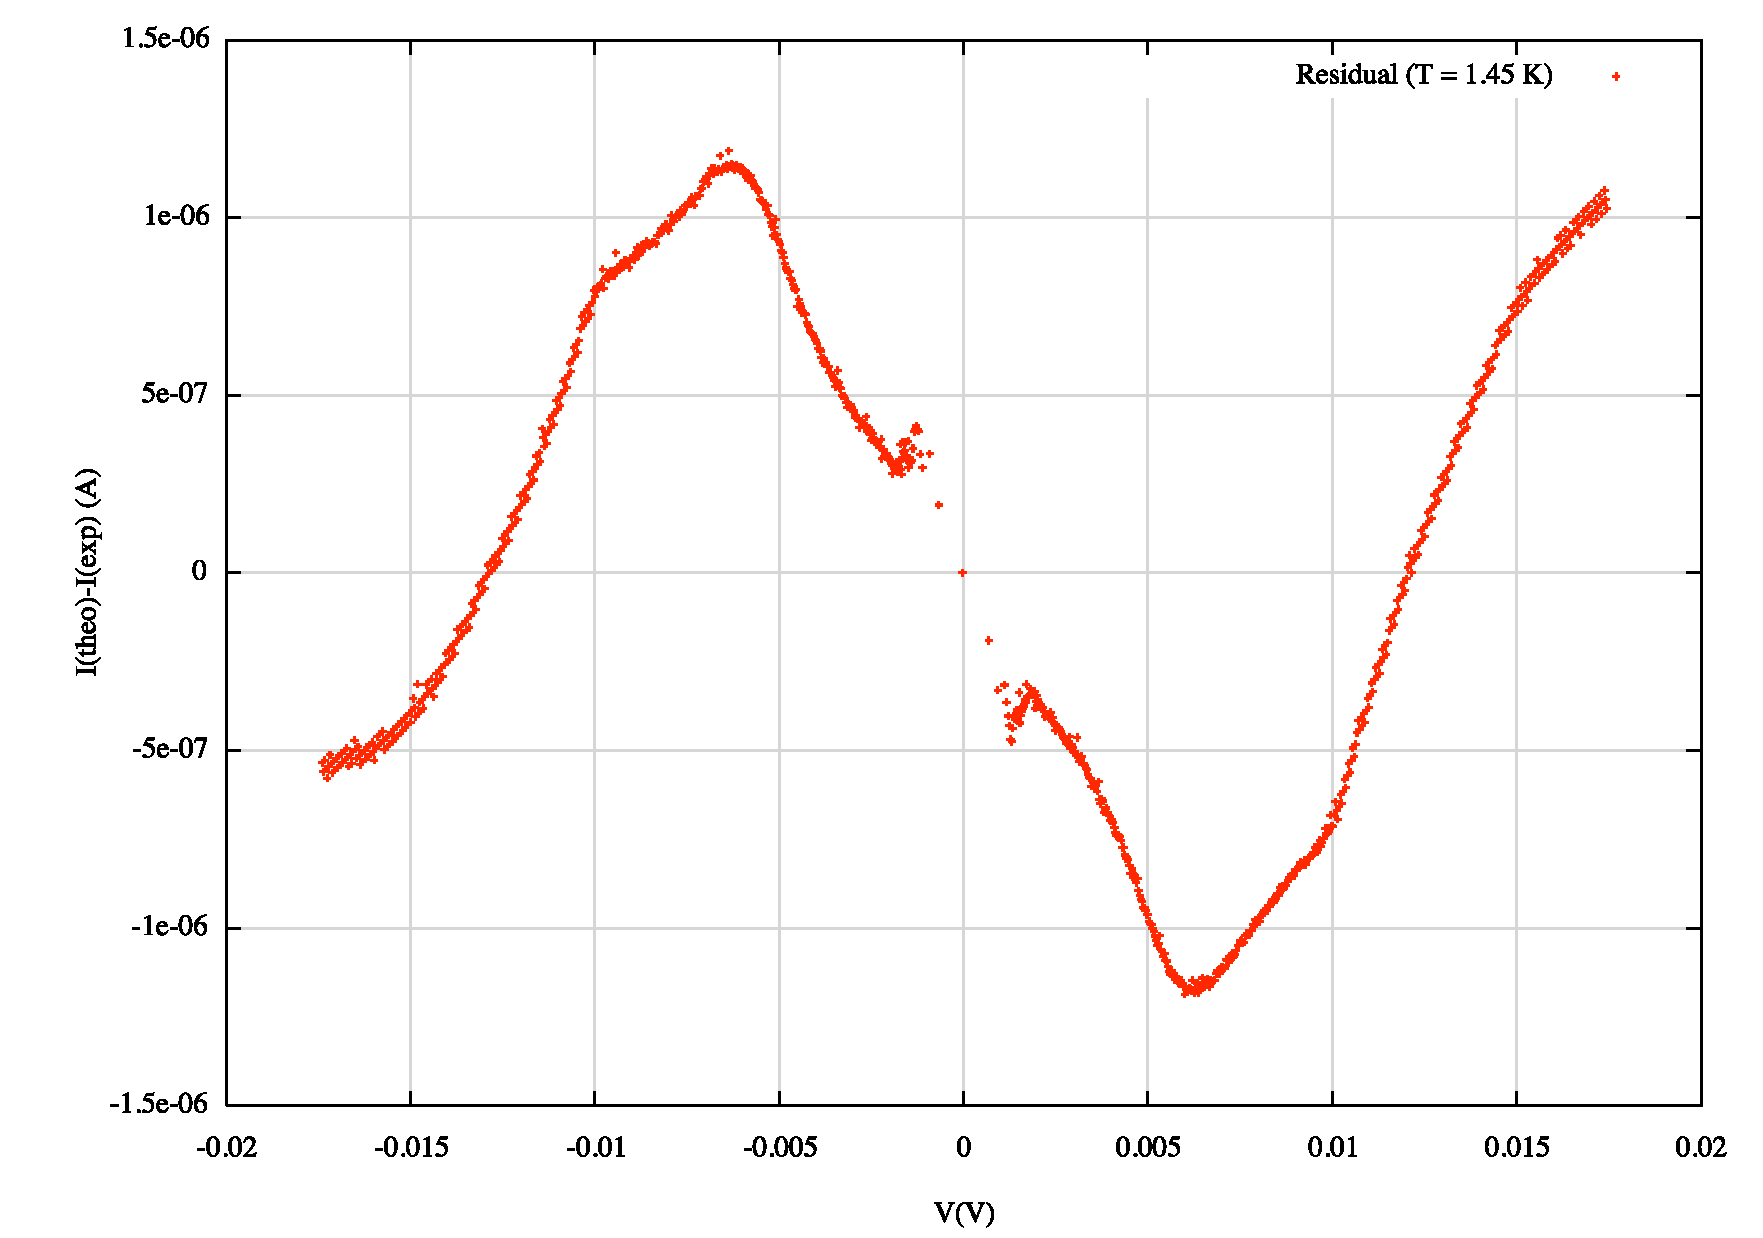
\includegraphics[width=0.45\textwidth]{residual}
\caption{\small Residual between theoretical and experimental current curve for $1.45 K$. The phonon structure arises clearly. 
\label{residual}}
\end{figure}


Our best guess as to what might be causing this effect is electron-phonon scattering. It seems not to vary significantly with Temperature (see fig. \ref{gv_3-4-5-7}) in the range of our observations. The shape of the deviation from the current predicted by BCS theory can be seen in figure \ref{residual}. Giaver also reports the same effect in a later paper \cite{giaever2}, and suggests it can be accounted for using a non-constant energy-gap parameter.

The initial idea for estimating the energy gap and the other parameters of the model($T$,$C_{NN}$) was to fit them using a least squares method. We tried to do so using a Levenberg-Marquard routine. This approach proved inefficient, with the results being rather dependent on the initial guess, and convergence reached at unexpected values. This is probably due to the algorithm over-fitting in the region affected by the model insufficiencies described above, as well as the high degree of nonlinearity exhibited by the function.

A more feasible method was to estimate normal-normal conductance and temperature from other measurements, and then fitting the value of the gap "by hand".

\begin{figure}[h!]
\centering
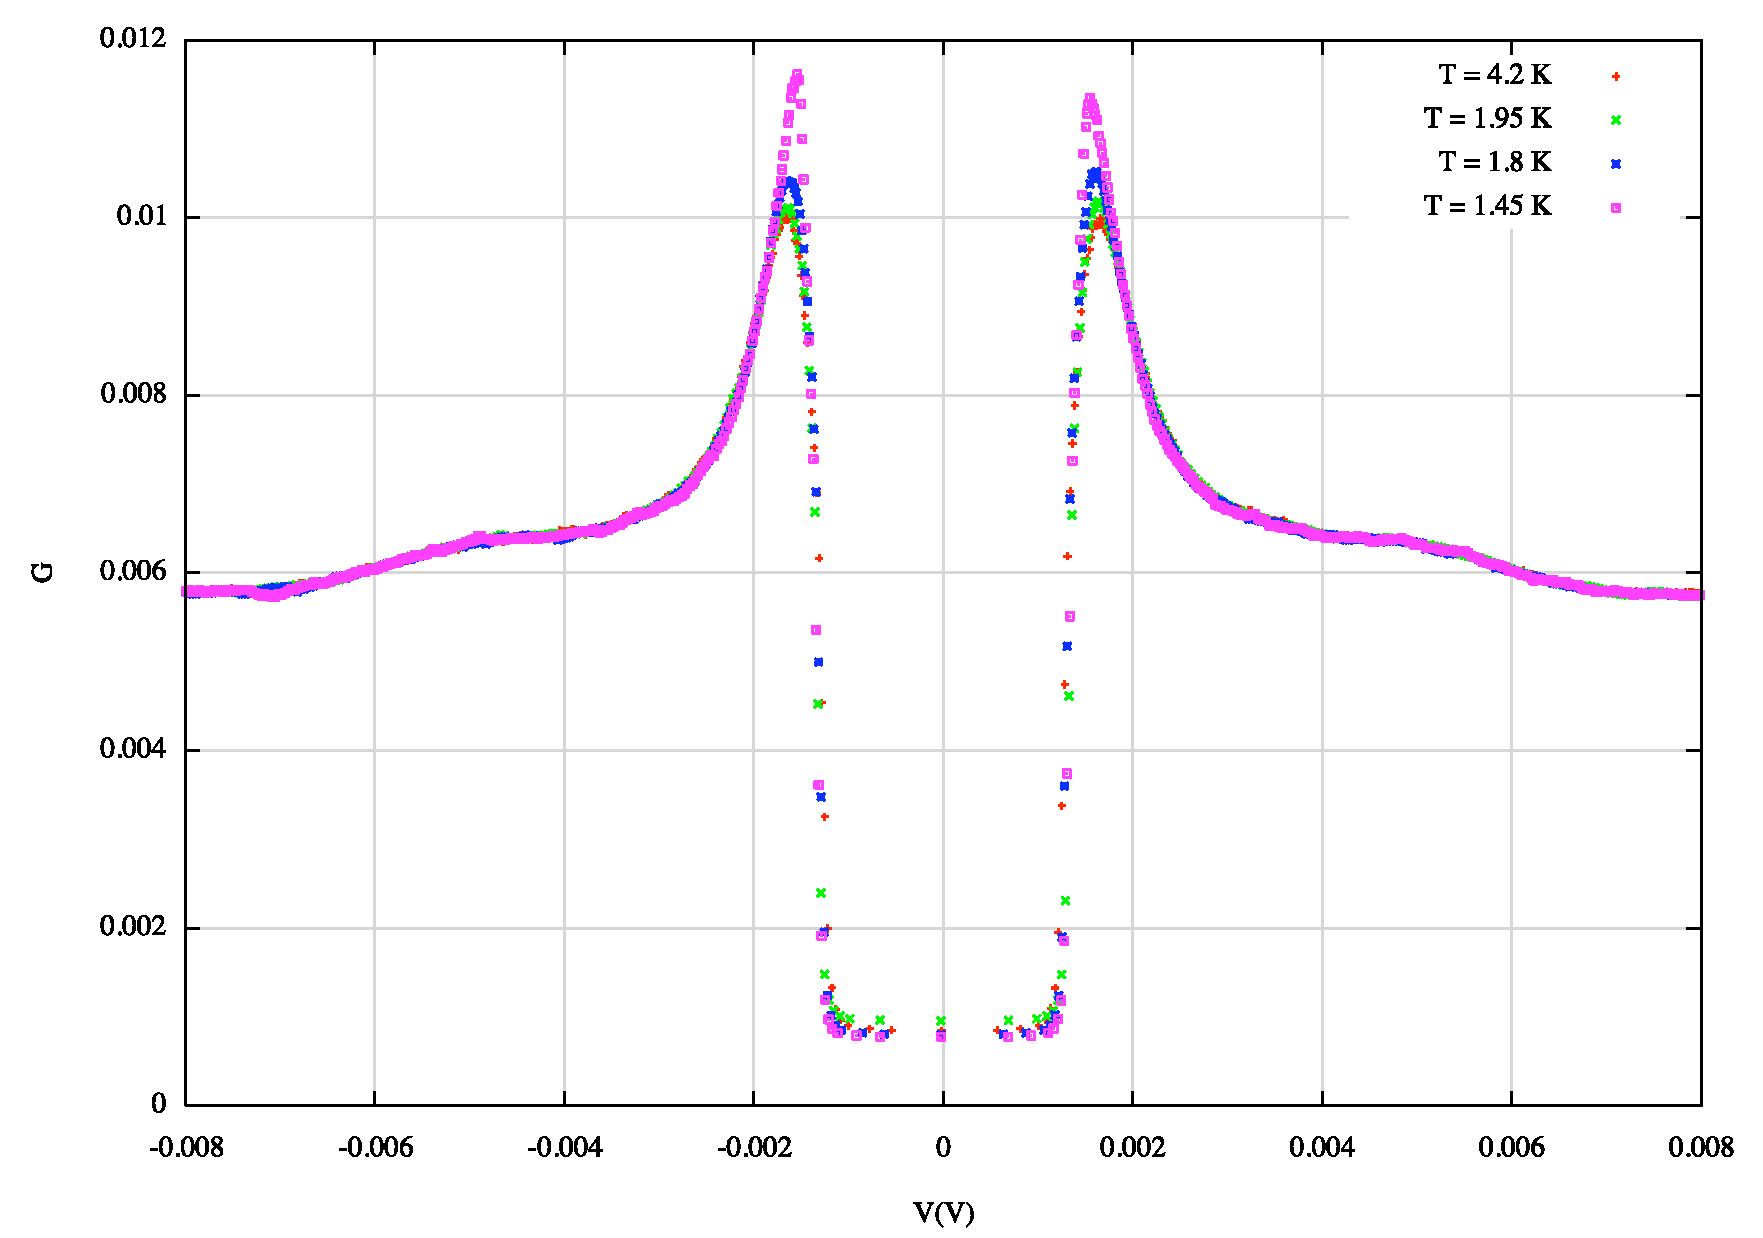
\includegraphics[width=0.45\textwidth]{gv_3-4-5-7}
\caption{\small Measured conductance for 4 different temperatures. The peaks coincidence sustains the nearly invariance of the gap for this temperature range. The phonon structure is the same for all.
\label{gv_3-4-5-7}}
\end{figure}


\subsection{Results}

\begin{figure}[h!]
\centering
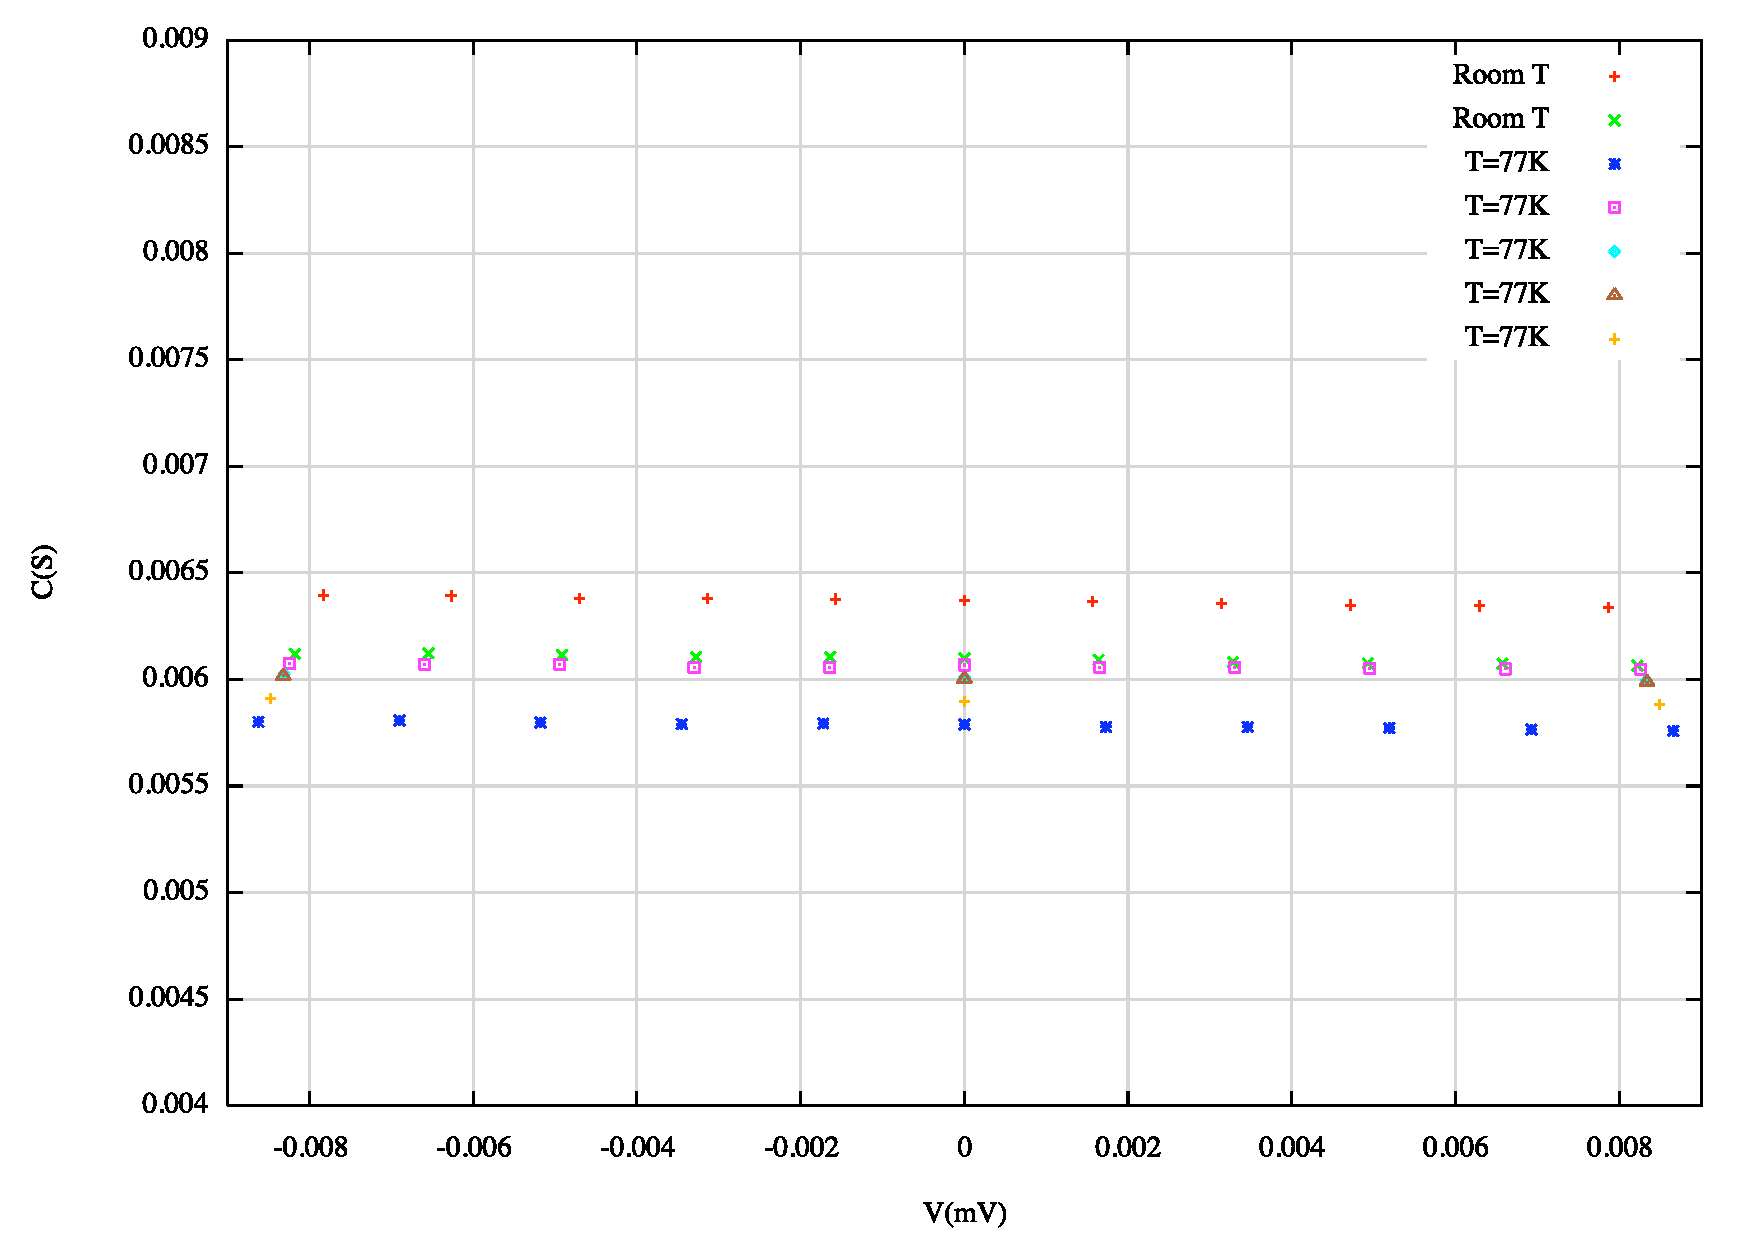
\includegraphics[width=0.45\textwidth]{conductance2}
\caption{\small Conductance curves . \label{conductance2}}
\end{figure}

Prior to inserting He into the cryostat as described, we measured the conductivity of the sample several times at different temperatures. From these measurements we determined $C_{NN}=0.006\pm0.0005 S$. The values taken in the relevant range of voltages can be seen in  fig. \ref{conductance2}.

%----------------------
%	2nd : T by helium vapor pressure --> manometer�?�? error??? 
The values for the Temperature were obviously different for each measurement. We determined it by means of associating temperatures to pressures at the surface of the $He^4$ using the vapor pressure curve. As described earlier, there was a manometer connected to the cryostat, and readings were taken at every measurement. This assumes that the pressure is nearly the same at the surface and at the top of the cryostat, where the measurement is taken.

The manometer is at room temperature while the temperature at the bottom of the cryostat is below $4.2 K$, so we have a temperature gradient. There exists in the cryostat's tube a thermomolecular pressure gradient between the hot (higher pressure) and cold (lower pressure) extremes that is sizeable when the mean free path of the molecules is not much smaller than the tube diameter. When the effect is not measured, one usually corrects for this gradient using the Weber-Schmidt equation \cite{weber}, although also the experimental tables of Roberts and Sydoriak \cite{roberts} or the calculation of Bennett and Tompkins can be used.

We do not need to do so because the Knudsen number, i.e. the ratio between molecular mean free path $\lambda$ and representative physical length $L$ (diameter of the cryostat), is small for our experimental layout:
\begin{equation}\label{knudsen}
K_n = \frac{\lambda}{L} =\frac{1}{L}\frac{RT}{\sqrt{2}\pi d^2 N_A P} << 1,
\end{equation}
where $d$ is the diameter of molecules.



%---------------------
The measurements from the manometer might also have been faulty, the pressure shown at room pressure was too low (700 mbar). The difference caused by this miscalibration seemed to be very low at lower pressures, of about 5 mbar, and hence less than $0.1\ K$.

\begin{table}[h]
\caption{\small Vapor pressures and corresponding temperatures of our measurements.}
\begin{center}
\begin{tabular}{c|c}
$p_{He}(mbar)$&$T(K)$\\
\hline
25	&	2.02	\\
14	&	1.83	\\
2	&	1.39	\\
$<1$	&	$<1.27$\\
\end{tabular}
\end{center}
\label{default}
\end{table}%


\begin{figure}[h!]
\centering
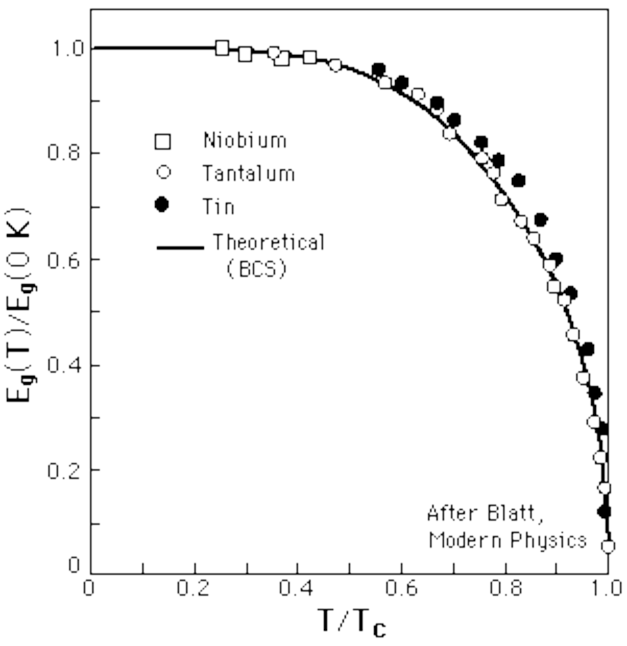
\includegraphics[width=0.45\textwidth]{bcs_gap2}
\caption{\small Reduced values of the observed energy gap as a function of the reduced temperature, after Towsend and Sutton. The solid curve is drawn for the BCS theory. \label{bcs_gap2}}
\end{figure}

With the other parameters now fixed, the width of the energy gap can now be fitted. Theoretically it depends on the temperature, but in the range of temperatures we measured in this change is very small, as can be seen in figure \ref{bcs_gap2}. The amount of change for temperatures between $1.2\ K$ and $4.2\ K$ is $\approx 0.07\Delta_0$, which is about $0.1 meV$, the error we expected to be caused by our fitting of the value "by hand", and we consequently assumed the value to be the same in all the measurements. Fitting the width by this process for the different measurements gave us a value of  $1.4\pm0.1$ meV. The error is a rough estimate based on the finesse with which we manually adjusted the gap. It is probably a little to large, yet we decided to give this slightly higher figure to account for the uncertainties in the temperature.

\begin{figure}[h!]
\centering
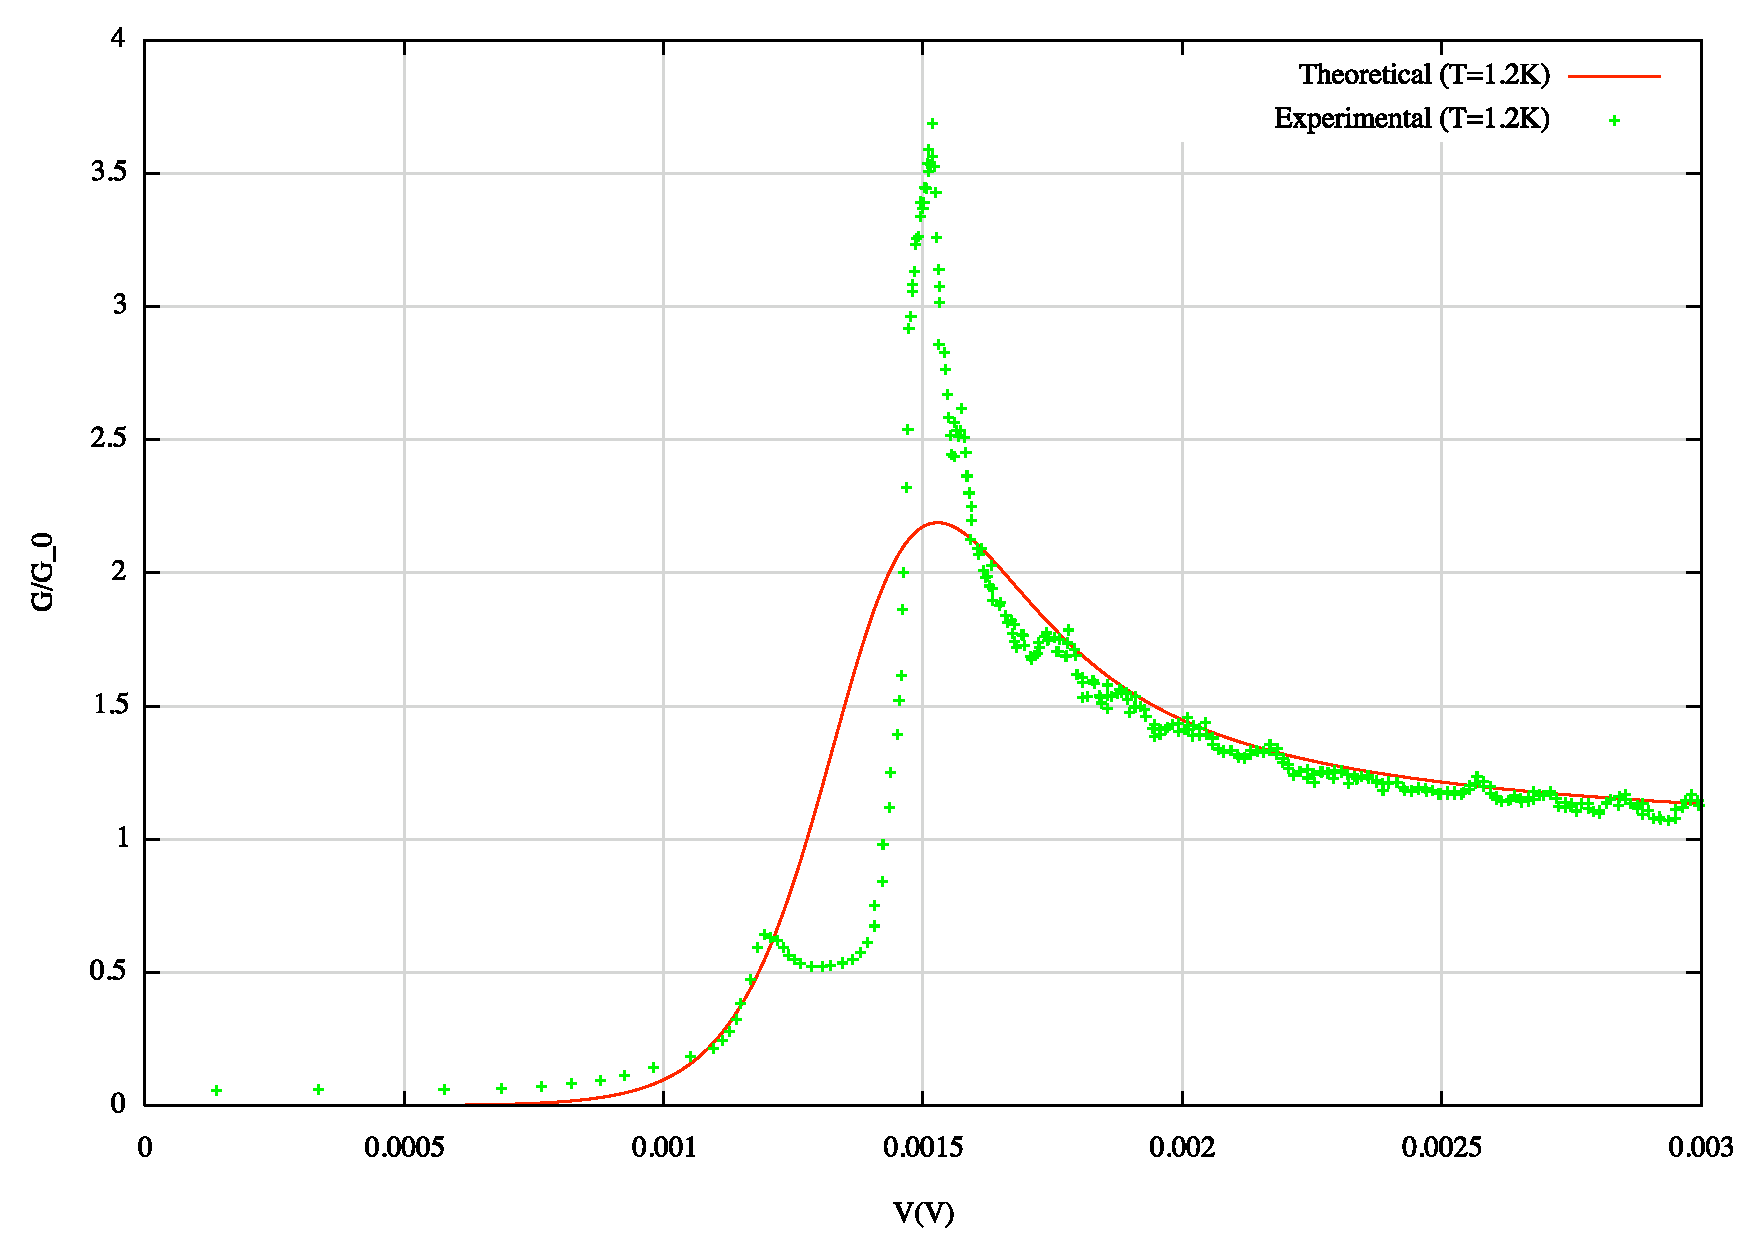
\includegraphics[width=0.45\textwidth]{gv_theo_exp_10}
\caption{\small Experimental data and BCS theoretical prediction for $1.2 K$. There is a second peak due to the superconductor transition of some parts of the Aluminum.
\label{gv_theo_exp_10}}
\end{figure}

The measurement at the lowest temperature we could perform gives qualitatively different results. In fig. \ref{gv_theo_exp_10} can be seen the appearance of new effects. The transition temperature $T_c$ for Aluminum is $1.140 K$, and we have established experimentally the temperature for data as $1.2 K$. However, due to the difference between bulk properties and those that we must consider here for thin films, the $T_c$ is a little bit greater (see \cite{films}).

The situation is qualitatively clear now, i.e. the temperature has fallen enough to let some portions of Aluminum change to superconducting state, creating this combined effect between normal-superconductor and superconductor-superconductor junctions. It can be explained by considering a sum of junctions of these two kinds in parallel, so as to produce an I-V curve with peaks inside the gap of the Aluminum. For a superconductor-superconductor junction appear two peaks, located at $| \Delta_1-\Delta_2|$ and $(\Delta_1+\Delta_2)$.








%-----------------------------------------------------------------
%-----------------------------------------------------------------
%-----------------------------------------------------------------
%-----------------------------------------------------------------
\begin{thebibliography}{99}

\bibitem{giaever1} I. Giaever and K. Megerle, \emph{Study of Superconductors by Electron Tunneling}, Phys. Rev. vol. 122, Num. 4, p. 1101 (1961)

\bibitem{giaever2} I. Giaever, \emph{Electron Tunneling and Superconductivity}, Rev. Mod. Phys. vol. 48, Num. 2, (1974)

\bibitem{giaever3} I. Giaever, \emph{Energy Gap in Superconductor Measured by Electron Tunneling}, Phys. Rev. Let. vol. 5, Num. 4, p. 147 (1960)

\bibitem{frerichs} R. Frerichs and J. P. Wilson, \emph{Tunnel-Effect Measurements on Superimposed Layers of Lead and Aluminum}, Phys. Rev. vol. 142, Num. 1, p. 264 (1966)

\bibitem{bcs} J. Bardeen, L. N. Cooper and J. R. Schrieffer, \emph{Theory of Superconductivity}, Phys. Rev. vol. 108, Num. 5, p. 1175 (1957)

\bibitem{ashcroft} N. W. Ashcroft and N. D. Mermin, \emph{Solid State Physics}, Harcourt College Publishers (1976)

\bibitem{formulas} Jianping Li, \emph{General explicit difference formulas for numerical differentiation}, Journal of Computational and Applied Mathematics vol. 183, p. 29 (2005)

\bibitem{films} M. Strongin, O. F. Kammerer & A. Paskin, \emph{Superconducting Transition Temperature of Thin Films},  Phys. Rev. Lett. 14, p. 949 - 951 (1965)

\bibitem{recipes} W. H. Press, S. A. Teukolsky, W. T. Vetterling and B. P. Flannery \emph{Numerical Recipes},  Cambridge University Press (1997)



\end{thebibliography}

%-----------------------------------------------------------------
%-----------------------------------------------------------------
%-----------------------------------------------------------------
\ednotemessage
%-----------------------------------------------------------------
\end{document}